 \documentclass[a4paper,12pt]{book}
\usepackage{multirow}
\usepackage{ZeroSeven}
\usepackage{ltablex}
\usepackage{graphicx}

\titlepage{}

\author{Mirko Franco}
\date{26-11-2018}
\intestazioni{
\includegraphics[scale=0.3]{images/logo_intestazione}}
\pagestyle{myfront}
\begin{document}
\begin{titlepage}
	\centering
	{\huge\bfseries MegAlexa\par}
	Arricchitore di skill di Amazon Alexa
	\line(1,0){350} \\
	{\scshape\LARGE Piano di Progetto \par}
	\vspace{1cm}
	{\scshape Gruppo ZeroSeven \par}
	\logo
	%devono essere compilati questi campi ogni volta
	\begin{tabular}{c|c}
		{\hfill \textbf{Versione}} 			& 0.0.2				\\
		{\hfill\textbf{Data Redazione}} 	& 26-11-2018		\\ 
		{\hfill\textbf{Redazione}} 			&  		Mirko Franco			\\ 
		{\hfill\textbf{Verifica}} 				&  	Bianca Ciuche				\\ 
		{\hfill\textbf{Approvazione}} 		&  		Mirko Franco			\\ 
		{\hfill\textbf{Uso}} 					& 		Esterno		\\ 
		{\hfill\textbf{Distribuzione}} 			& 			Prof. Tullio Vardanega \\ & Prof. Riccardo Cardin \\ & Gruppo ZeroSeven		\\ 
		{\hfill\textbf{Email di contatto}} & zerosevenswe@gmail.com \\
	\end{tabular}
\end{titlepage}
	\label{LastFrontPage}
	\newpage	
	\begin{center}
	\textbf{Registro delle modifiche}
	\end{center}
	\begin{center}
		\begin{tabularx}{\textwidth}{|c|c|X|X|c|}
			\hline
			\textbf{Versione} & \textbf{Data} & \textbf{Descrizione} & \textbf{Autore} & \textbf{Ruolo} \\ 
			\hline
			3.0.0 & 2019-04-11 & Approvazione per il rilascio RQ & Ludovico Brocca & Responsabile \\
			\hline
			2.1.0 & 2019-04-09 & Verifica documento & Ludovico Brocca & Verificatore \\
			\hline
			2.0.6 & 2019-04-08 & Aggiunto riferimento metriche alla sezione \S\ref{MetricheObbiettivi} &Matteo depascale & Amministratore \\
			\hline 
			2.0.5 & 2019-04-08 & Modifica sezioni \S\ref{Verifica}  e \S\ref{Validazione} & Matteo depascale & Amministratore \\
			\hline
			2.0.4 & 2019-04-08 & Aggiunti comandi personalizzati alla sezione \S\ref{NormeRedazionali} &Matteo depascale & Amministratore \\
			\hline
			2.0.3 & 2019-04-04 & Aggiunta voci a \S\ref{ListaControllo} & Matteo depascale & Amministratore \\
			\hline
			2.0.2 & 2019-04-01 & Stesura sezioni \S\ref{DiagrammiDelleClassi}, \S\ref{DiagrammiPackage}, \S\ref{DiagrammiSequenza} e \S\ref{DiagrammiAttivita}  & Bianca Andreea Ciuche & Amministratore \\
			\hline
			2.0.1 & 2019-03-23 & Modifica \ref{Documentazione fornita} Corretti numeri di sezione & Bianca Andreea Ciuche & Amministratore \\
			\hline
			2.0.0 &2019-03-07 & Approvazione per il rilascio & Gian Marco Bratzu& Responsabile\\
			\hline
			1.2.0 &2019-03-02 & Verifica documento &Andrea Deidda& Verificatore\\
			\hline
			1.1.2 &2019-02-13 &Stesura \S\ref{calcoloOre} &Ludovico Brocca& Amministratore\\
			\hline
			1.1.1 &2019-02-13 &Modifica\S \ref{anDinamica} &Ludovico Brocca& Amministratore\\
			\hline
			1.1.0 &2019-02-07 &Verifica \S\ref{processo}, \ref{metriche}, \S\ref{progettazione} &Gian Marco Bratzu& Verificatore\\
			\hline
			1.0.4 &2019-02-04&Stesura \S\ref{processo}&Ludovico Brocca& Analista\\
			\hline
			1.0.3 & 2019-02-03 & Modifica \S\ref{metriche} & Stefano Zanatta & Amministratore\\
			\hline
			1.0.2 & 2019-02-02 & Stesura \S\ref{metriche} & Bianca Andreea Ciuche & Amministratore\\
			\hline
			1.0.1 & 2018-01-12 & Stesura \S\ref{progettazione} & Mirko Franco & Amministratore \\
			\hline
			1.0.0 & 2018-01-09 & Approvazione per il rilascio & Stefano Zanatta & Responsabile\\
			\hline
			0.2.0 & 2018-12-29 & Verifica documento & Stefano Zanatta & Verificatore\\
			\hline
			0.1.0 & 2018-12-18 & Verifica \S\ref{PdS} & Mirko Franco & Verificatore\\
			\hline
			0.0.6 & 2018-12-21 & Modifica \S\ref{Intro} & Andrea Deidda & Amministratore\\
			\hline
			0.0.5 & 2018-12-17 & Stesura \S\ref{Po} & Ludovico Brocca & Amministratore\\
			\hline
			0.0.4 & 2018-12-16 & Stesura \S\ref{Pp} & Matteo Depascale & Amministratore\\
			\hline
			0.0.3 & 2018-12-16 & Stesura \S\ref{Intro} & Bianca Ciuche & Amministratore\\
			\hline
			0.0.2 & 2018-12-10 & Stesura \S\ref{PdS} & Gian Marco Bratzu & Amministratore\\	
			\hline
			0.0.1 & 2018-12-08 & Struttura documento  & Ludovico Brocca & Amministratore\\
			\hline
	\end{tabularx}
	\end{center}

\newpage
	\pagestyle{mymain}
	\tableofcontents
	\listoftables
	\listoffigures
	\chapter{Organigramma}
\label{organigramma}
\section{Redazione}
\label{redazione}
	\begin{table}[htp]
		\centering
			\begin{tabular}{|c|c|c|}
				\hline
				\textbf{Nominativo} & \textbf{Data di redazione} & \textbf{Firma} \\
				\hline 
				Mirko Franco & 2018-11-26 &  \\
				\hline
			\end{tabular}
				\caption{Redazione}
	\end{table}
\section{Approvazione}
\begin{table}[htp]
	\centering
	\begin{tabular}{|c|c|c|}
		\hline
		\textbf{Nominativo} & \textbf{Data di approvazione} & \textbf{Firma} \\
		\hline 
		Mirko Franco & 2019-01-09 &  \\
		\hline
	\end{tabular}
	\caption{Approvazione}
\end{table}
\clearpage
\section{Accettazione dei componenti}
\label{accettazione}
\begin{tabularx}{\textwidth}{|c|c|c|}
			\hline
			\textbf{Nominativo} & \textbf{Data di accettazione} & \textbf{Firma} \\
			\hline 
			Gian Marco Bratzu & 2019-01-10 & \\
			Ludovico Brocca & 2019-01-10 & \\
			Bianca  Andreea Ciuche & 2019-01-10 & \\
			Andrea Deidda & 2019-01-10 & \\
			Matteo Depascale & 2019-01-10 & \\
	 		Mirko Franco & 2019-01-10 &  \\
	 		Stefano Zanatta & 2019-01-10 & \\
			\hline
		\caption{Accettazione dei componenti}
\end{tabularx}


\section{Componenti}
\label{componenti}
		\begin{tabularx}{\textwidth}{|X|X|c|X|}
			\hline
			\textbf{Nome e Cognome} &\textbf{Matri-}\newline \textbf{cola} & \textbf{Indirizzo di posta elettronica} \\
			\hline 
			Gian Marco Bratzu & 1049631 &gianmarco.bratzu@studenti.unipd.it \\
			\hline
			Ludovico Brocca & 1123298 & ludovico.brocca@studenti.unipd.it \\
			\hline
			Bianca Andreea Ciuche & 1122193 & biancaandreea.ciuche@studenti.unipd.it \\
			\hline
			Andrea Deidda & 1144405 & andrea.deidda@studenti.unipd.it \\
			\hline
			Matteo Depascale & 1120162 & matteo.depascale@studenti.unipd.it \\
			\hline
			Mirko Franco & 1138070 &  mirko.franco.1@studenti.unipd.it \\
			\hline
			Stefano Zanatta & 1142897 & mail@studenti.unipd.it \\
			\hline
			\caption{Componenti}
		\end{tabularx}
			

\section{Assunzioni sui ruoli}
	Durante tutta la durata del progetto i componenti del gruppo sono tenuti a ricoprire dei ruoli chiave per la buona riuscita dello stesso.
	Tali ruoli sono descritti in modo approfondito nelle \textit{Norme di Progetto v1.0.0} e di seguito riportati:
	\begin{itemize}
		\item \textit{Responsabile};
		\item \textit{Amministratore};
		\item \textit{Analista};
		\item \textit{Progettista};
		\item \textit{Programmatore};
		\item \textit{Verificatore}.
	\end{itemize}
	\begin{comment}
		
	Ciascun ruolo ha un diverso costo. Di seguito verrà riportato, per ogni ruolo, il suo costo orario:

		\begin{tabularx}{\textwidth}{|c|c|}
			\hline
			\textbf{Ruolo} & \textbf{Costo} \\
			\hline
			Responsabile & 30 \euro \\
			Amministratore & 20 \euro \\
			Analista & 25 \euro \\
			Progettista & 22 \euro \\
			Programmatore & 15 \euro \\
			Verificatore & 15 \euro \\
			\hline
			\caption{Costi per ruolo}
		\end{tabularx}

	\end{comment}
	\chapter{Introduzione}
\label{introduzione}
\section{Scopo del documento}
Il \textit{Piano di Qualifica} ha lo scopo di definire gli obbiettivi di qualità che il gruppo perseguita per il proprio prodotto. Per ottenere tali obbiettivi è necessario un processo di verifica continua di ogni attività. Questo consente di rilevare e correggere le anomalie riscontrate tempestivamente.\\
Questo documento descrive nel dettaglio la qualità dei processi più vicini nel tempo e ad alto livello quelli più lontani, per poi essere aggiornato con nuovi contenuti ogni volta che il gruppo lo ritiene necessario.
\section{Scopo del prodotto}
Lo scopo del progetto è quello di sviluppare un applicativo Mobile in grado di creare delle routine personalizzate per gli utenti gestibili tramite\glossario{Alexa}di\glossario{Amazon}. L'obbiettivo è quello di creare\glossario{skill}in grado di avviare\glossario{workflow}creati dagli utenti fornendogli dei\glossario{connettori}.
\section{Glossario}
Al fine di evitare ogni ambiguità di linguaggio e massimizzare la comprensione dei documenti, i termini tecnici, di dominio, gli acronimi e le parole che necessitano di essere chiarite, sono riportate nel \textit{Glossario v1.0.0}.\\
Ogni occorrenza di vocaboli presenti nel \textit{Glossario} è marcata da una "G" maiuscola in pedice.
\section{Riferimenti}
\subsection{Normativi}
\begin{itemize}
	\item  \textbf{Norme di Progetto}: \textit{Norme di Progetto v1.0.0};
	\item \textbf{Capitolato$_{G}$ C4}:\glossario{MegAlexa}: arricchitore di skill di Amazon Alexa.
	\item \textbf{Ciclo di Deming}
	\footnote{\url{https://it.wikipedia.org/wiki/Ciclo_di_Deming}}
\end{itemize}
\subsection{Informativi}\label{rfinf}
\begin{itemize}
	\item \textbf{Piano di Progetto}: \textit{Piano di Progetto v1.0.0};
	\item \textbf{Complessità ciclomatica}
	\item \textbf{Software Testing Fundamentals: Methods and Metrics} di Marnie L. Hutcheson, Wiley Publishing, Inc.  
	\footnote{\url{https://www.math.unipd.it/~tullio/IS-1/2018/Progetto/C4.pdf}}.
	
	
\end{itemize}

	\chapter{Pianificazione}
Lo sviluppo del progetto è diviso in cinque periodi:
\begin{itemize}
    \item \textbf{Analisi} AN;
    \item \textbf{Analisi Dettaglio} AD;
    \item \textbf{Progettazione Architetturale} PA;
    \item \textbf{Progettazione di Dettaglio e Codifica} (PDC);
    \item \textbf{Validazione} (VV);
\end{itemize}
In ogni periodo sono presenti delle attività da svolgere, alle quali sono associate una o più risorse. Ogni attività è sottoposta a verifica, per semplificare il processo di Validazione.\\
Le attività sono suddivise in più sotto-attività.\\
Nel Gantt$_{G}$ vengono riportate:
\begin{itemize}
    \item \textbf{attività:} contengono più sotto-attività. Nel Gantt$_{G}$ sono rappresentate con una linea grigia.
    \item \textbf{milestone$_{G}$:} rappresenta la data ultima prevista per il completanento di un insieme prestabilito di attività. Ha durata di 0 (zero) giorni e coincide con la data della successiva revisione o l'approvazione complessiva di tali attivita. È rappresentata nel $_Gantt$ con un rombo nero;
    \item \textbf{sotto-attività:} attività atomiche che possono essere svolte da una persona. Nel Gantt$_{G}$ sono rappresentate con una linea blu.  
\end{itemize}
\section{Analisi}
\textbf{Periodo:} da 2018-11-25 a 2019-01-21\\L'Analisi inizia in concomitanza con la pubblicazione dei capitolati d’appalto e termina alla Revisione dei Requisiti (RR).\\
Le attività della fase di Analisi sono:
\begin{itemize}
    \item \textbf{Studio di Fattibilità:} vengono valutati tutti i capitolati d'appalto, la valutazione è basata sull'interesse personale di ogni membro del gruppo, sulla complessità prevista, sui rischi che possono emergere. Viene data anche data una descrizione generale del capitolato e una analisi preliminare.\\Viene svolta come prima attività, in quanto bloccante per l'Analisi dei requisiti;
    \item \textbf{Norme di Progetto:} le norme di progetto contengono le regole che il gruppo dovrà seguire durante l'attuazione di tutte le attività. I verificatori certificheranno il rispetto delle norme;
    \item \textbf{Analisi dei Requisiti:} l'analisi preliminare nello Studio di Fattibilità viene approfondita.\\Tale attività continuerà sino alla data di consegna;
    \item \textbf{Piano di Progetto:} Il Responsabile del gruppo redige il piano di progetto, rispettando i vincoli posti dal proponente.\\Questo documento ha l'obiettivo di regolare le attività svolte dal gruppo;
    \item \textbf{Piano di qualifica:} Il piano di qualifica contiene le strategie utili al raggiungimento degli obiettivi del proponente, del gruppo e inerenti alla qualità dei processi di sviluppo.\\L'obiettivo è quello di rendere la qualità quantificabile e misurabile;
    \item \textbf{Glossario:} scritto in modo incrementale. Contiene la spiegazione dei termini più tecnici utilizzati nei documenti. Questa attività è svolta da tutti i membri del gruppo, in parallelo con la redazione di tutti i documenti.
    \item \textbf{Lettera di presentazione:} documento presentato al committente che permette al gruppo di partecipare alla gara d’appalto per il capitolato.
\end{itemize}
I ruoli maggiormente coinvolti sono: Responsabile, Amministratore e Analista.
\section{Analisi Dettaglio}
\textbf{Periodo:} da 2019-01-21 a 2019-02-15\\
L'\textbf{Analisi Dettaglio} inizia dopo la \textbf{Revisione dei Requisiti} e termina con l’inizio della \textbf{Progettazione Architetturale}. Questo periodo viene utilizzato dal team per consolidare i requisiti richiesti dal sistema e per migliorare i documenti già redatti. In questo periodo i ruoli maggiormente coinvolti sono: \textbf{Responsabile}, \textbf{Amministratore} e \textbf{Analista}.

\section{Progettazione Architetturale}
\textbf{Periodo:} da 2019-02-15 a 2019-03-15\\
La Progettazione Architetturale inizia al termine dell’\textbf{Analisi Dettaglio} e termina con la consegna del prodotto alla \textbf{Revisione di Progetto}.\\
Le attività della fase di \textbf{Progettazione Architetturale} sono:
\begin{itemize}
    \item \textbf{Specifica Tecnica}: il Progettista del gruppo espone le scelte progettuali, ad alto livello, che il prodotto dovrà avere. Verranno descritti i design pattern utilizzati nella creazione del prodotto, l’architettura generale del software, i principali flussi di controllo e il tracciamento dei requisiti;
    \item \textbf{Incremento e Verifica:} tutti i documenti verranno aggiornati in base ai risultati della \textbf{Revisione dei Requisiti}. 
\end{itemize}
I ruoli maggiormente coinvolti sono: Responsabile, Amministratore, Progettista, Verificatore e Analista.

\section{Progettazione di Dettaglio e Codifica}
\textbf{Periodo:} da 2019-03-15 a 2019-04-16\\
Questo periodo inizia dopo la \textbf{Revisione di Progetto} e termina con la consegna del prodotto alla \textbf{Revisione di Qualità}.\\Le attività della fase di Progettazione di Dettaglio e Codifica sono:
\begin{itemize}
    \item \textbf{Definizione di Prodotto:} Viene definita approfonditamente la struttura e le relazioni dei componenti del prodotto, basandosi sul documento di \textit{Specifica Tecnica};
    \item \textbf{Codifica:} i programmatori sviluppano quel che è riportato nella \textit{Definizione di Prodotto};
    \item \textbf{Incremento e Verifica:} tutti i documenti verranno aggiornati in base al risultato della Revisione di Progettazione.
\end{itemize}
I ruoli maggiormente coinvolti sono: \textit{Responsabile}, \textit{Amministratore}, \textit{progettista}, \textit{Verificatore} e \textit{Programmatore}.

\section{Validazione}
\textbf{Periodo:} da 2019-04-16 2019-05-17\\
Questo periodo inizia al termine della \textbf{Progettazione di Dettaglio e Codifica} e si conclude con la \textbf{Revisione di Accettazione}.\\Con la \textbf{Validazione} il team svolge le ultime attività di Verifica e prepara il sistema per la Validazione e il rilascio.\\
Le attività sono:
\begin{itemize}
    \item \textbf{Validazione del Sistema}: il sistema viene validato e collaudato, per dimostrare la sua conformità con le specifiche accordate con il proponente;
    \item \textbf{Incremento e Verifica}: tutti i documenti verranno aggiornati in base al risultato della Revisione di Qualifica.
\end{itemize}

	\chapter{Preventivo}
Di seguito viene riportato il preventivo per il progetto MegAlexa; esso si divide,per ogni periodo,in:
\begin{itemize}
	\item \textbf{Prospetto orario:} presenta la distribuzione oraria e la suddivisione nei ruoli per ogni membro del gruppo ZeroSeven;
	\item \textbf{Prospetto economico:}presenta le ore di impegno calcolate per i ruoli coinvolti ed il rispettivo costo;
\end{itemize}
La suddivisione oraria viene svolta avendo come riferimento le seguenti regole:
\begin{itemize}
	\item Ogni membro del gruppo deve coprire ogni ruolo almeno una volta durante il ciclo di sviluppo del prodotto;
	\item Il totale delle ore di lavoro dovrà essere equamente distribuito tra i membri;
	\item Non ci devono essere conflitti di interesse in cui un Verificatore debba controllare il proprio lavoro.
\end{itemize}
Le sigle utilizzate per i vari ruoli saranno:
\begin{itemize}
	\item \textbf{Re:} Responsabile di Progetto;
	\item \textbf{Am:} Amministratore;
	\item \textbf{An:} Analista;
	\item \textbf{Pt:} Progettista;
	\item \textbf{Pr:} Programmatore;
	\item \textbf{Ve:} Verificatore;
\end{itemize}

Per il preventivo si tiene conto che i periodi di Analisi dei Requisiti e di Analisi dei Requisiti di Dettaglio sono considerati di investimento del gruppo e  non a carico dei committente, per cui  le ore di impegno svolte durante questi non saranno conteggiate nelle ore totali da retribuire.

\newpage
\section{Analisi  dei Requisiti}
\subsection{Prospetto orario}
Il prospetto orario per il periodo di Analisi dei Requisiti è illustrato nella seguente tabella:
\begin{table}[!ht]
	\begin{center}  	
		\begin{tabular}{c}
			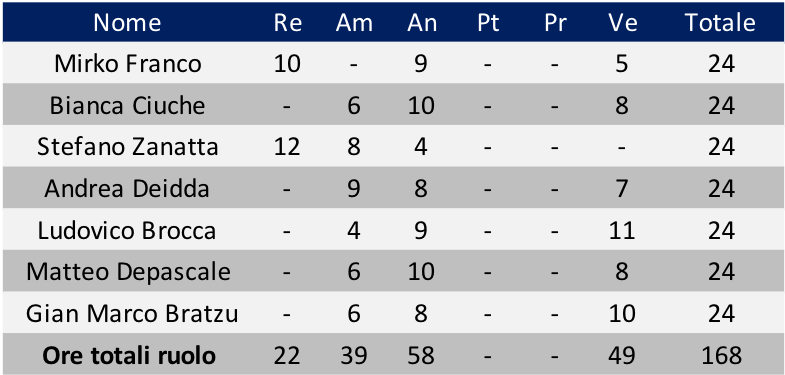
\includegraphics{images/tabellaProspettoOrario.png}
		\end{tabular}
		\caption{Prospetto Orario nel periodo di Analisi dei Requisiti}
	\end{center}
\end{table}

Il seguente grafico rappresenta la suddivisione oraria dei ruoli all'interno del gruppo:
\begin{figure}[!ht]
	\begin{center}
		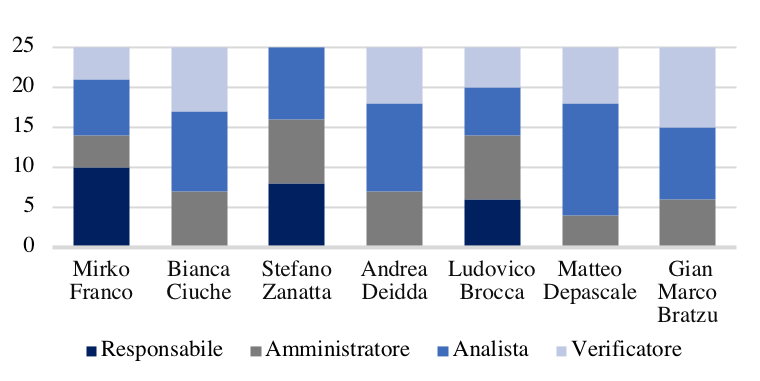
\includegraphics{images/grafoProspettoOrario.png}
		\caption{Grafico prospetto orario nel periodo di Analisi dei Requisiti }
	\end{center}
\end{figure}

\subsection{Prospetto Economico}
Il prospetto economico per il periodo di Analisi dei Requisiti è illustrato nella seguente tabella.
Le spese per questa attività non sono a carico del committente.

\begin{table}[!ht]
	\begin{center}
		\begin{tabular}{c}
			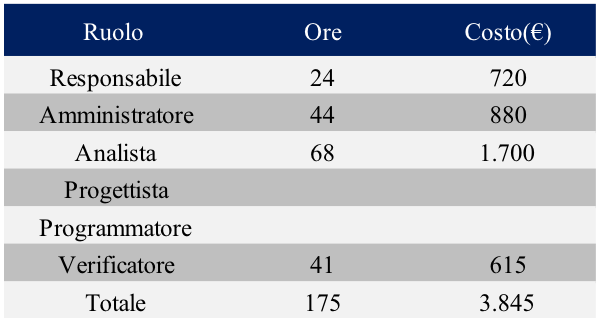
\includegraphics{images/tabellaProspettoEconomico.png}
		\end{tabular}
		\caption{Prospetto Economico nel periodo di Analisi dei Requisiti}
	\end{center}
\end{table}
La raffigurazione grafica del peso di ogni ruolo sul costo totale è così rappresentata:
\begin{figure}[!ht]
	\centering
	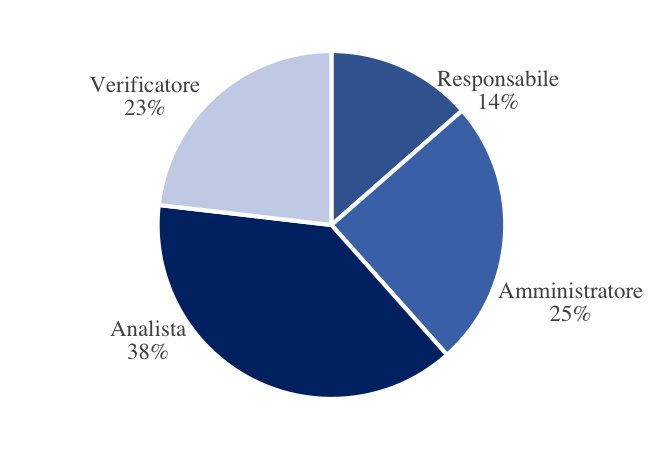
\includegraphics{images/grafoProspettoEconomico.png}
	\caption{Grafico prospetto economico nel periodo di Analisi dei Requisiti }
\end{figure}

\newpage
\section{Analisi dei Requisiti di Dettaglio}
\subsection{Prospetto Orario}
Il prospetto orario per il periodo di Analisi dei Requisiti di Dettaglio è illustrato nella seguente tabella:

\begin{table}[!ht]
	\begin{center}
		\begin{tabular}{c}
			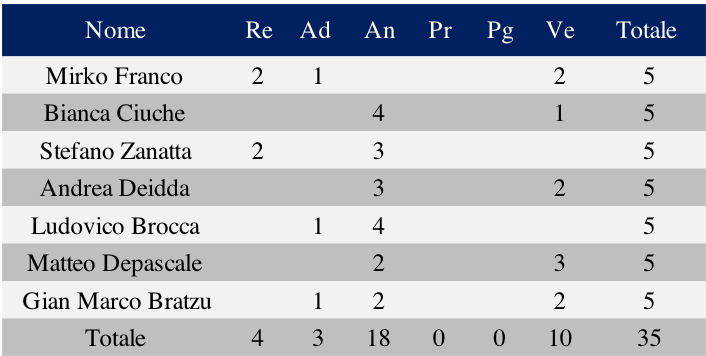
\includegraphics[scale=0.90]{images/tabellaProspettoOrarioDett.png}
		\end{tabular}
		\caption{Prospetto Orario nel periodo di Analisi dei Requisiti di Dettaglio}
	\end{center}
\end{table}
Il seguente grafico rapresenta la suddivisione oraria dei ruoli all'interno del gruppo:
\begin{figure}[!ht]
	\begin{center}
		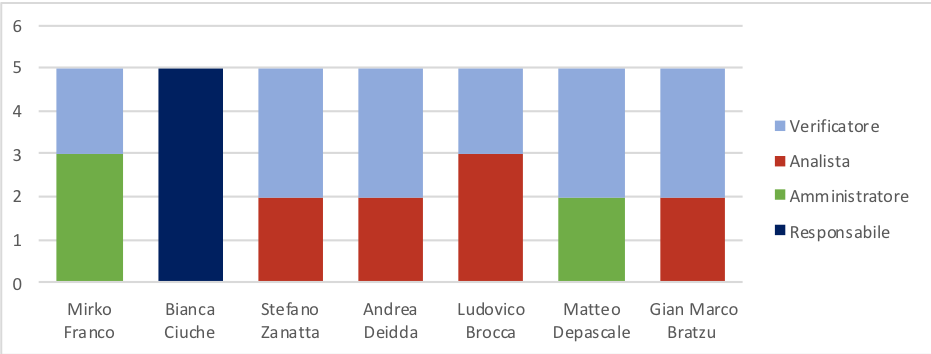
\includegraphics{images/grafoProspettoOrarioDett.png}
		\caption{Grafico prospetto orario nel periodo di Analisi dei Requisiti in Dettaglio}
	\end{center}
\end{figure}
\newpage
\subsection{Prospetto economico}
Il prospetto economico per il periodo di Analisi dei Requisiti di Dettaglio è illustrato nella seguente tabella.
Le spese per questa attività non sono a carico del committente.

\begin{table}[!ht]
	\begin{center}
		\begin{tabular}{c}
			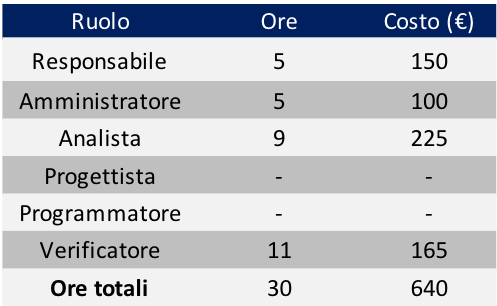
\includegraphics{images/tabellaProspettoEconomicoDett.png}
		\end{tabular}
		\caption{Prospetto Economico nel periodo di Analisi dei Requisiti di Dettaglio}
	\end{center}
\end{table}

La raffigurazione grafica del peso di ogni ruolo sul costo totale è così rappresentata:
\begin{figure}[!ht]
	\begin{center}
		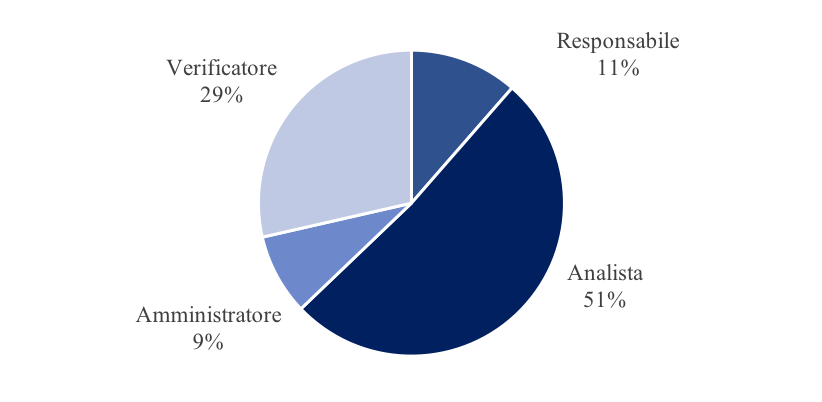
\includegraphics{images/grafoProspettoEconomicoDett.png}
		\caption{Grafico prospetto economico nel periodo di Analisi dei requisiti in dettaglio }
	\end{center}
\end{figure}

\newpage
\section{Progettazione della Base Tecnologica}
\subsection{Prospetto orario}
Il prospetto orario durante il periodo di Progettazione della Base Tecnologica è illustrato nella seguente tabella:

\begin{table}[ht]
	\caption{Prospetto Orario nel periodo di Progettazione della Base Tecnologica}
	\begin{center}
		\rowcolors{1}{}{lightgray}
		\begin{tabular}{ccccccccc}
			\rowcolor{lightblue}
			\hline
			& \textcolor{white}{Nome} & \textcolor{white}{Re} & \textcolor{white}{Am} & \textcolor{white}{An} & \textcolor{white}{Pt} &\textcolor{white}{Pr} & \textcolor{white}{Ve} & \textcolor{white}{Totale} \\
			\hline
			
			&Mirko Franco & - & 5 & 9 & 9 & 6 & - & 29  \\
			&Bianca Ciuche & -& - & 6 & 10 & - & 11 & 27 \\
			&Stefano Zanatta & 5 & - & - & 22 & - & - & 27 \\
			&Andrea Deidda &  -& - & - & 12 & 4 & 13 & 29 \\
			&Ludovico Brocca & -& 5 & - & 19 & 5 & - & 29 \\
			&Matteo Depascale & -& - & - & 11 & - & 18 & 29 \\
			&Gian Marco Bratzu & 7& - & - & 20 & - & - & 27 \\
			\hline
			&\textbf{Ore totali ruolo} & 12 & 10 & 15 & 103 & 15 & 42 & 197 \\
			
		\end{tabular}
	\end{center}
\end{table}

Il seguente grafico rapresenta la suddivisione oraria dei ruoli all'interno del gruppo:
\begin{figure}[!ht]
	\begin{center}
		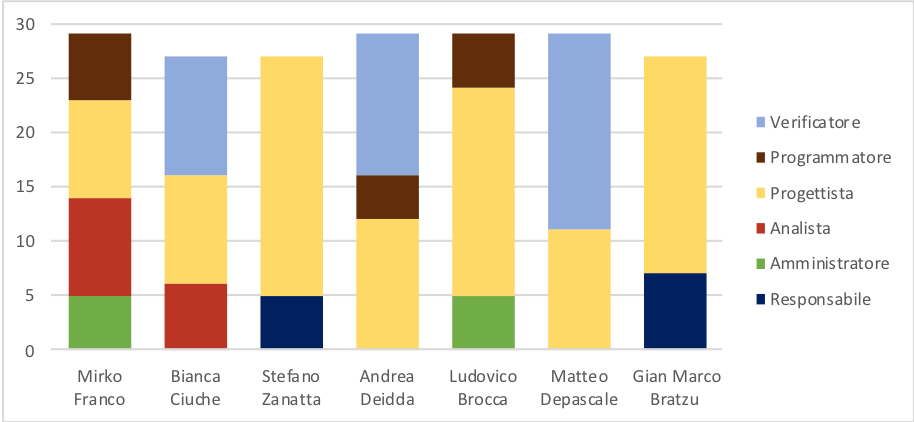
\includegraphics[scale=0.80]{images/grafoProgettazioneTecnologica.png}
		\caption{Grafico prospetto economico nel periodo di Progettazione della Base Tecnologica}
	\end{center}
\end{figure}
\newpage
\subsection{Prospetto economico}
Il prospetto economico per il periodo di Progettazione della Base Tecnologica è illustrato nella seguente tabella:

\begin{table}[!ht]
	\begin{center}
		\begin{tabular}{c}
			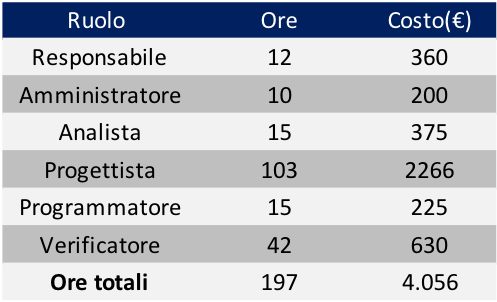
\includegraphics{images/tabellaProgettazioneTecnologicaEuro.png}
		\end{tabular}
		\caption{Prospetto Economico nel periodo di Progettazione della Base Tecnologica}
	\end{center}
\end{table}

La raffigurazione grafica del peso di ogni ruolo sul costo totale è così rappresentata:
\begin{figure}[!ht]
	\begin{center}
		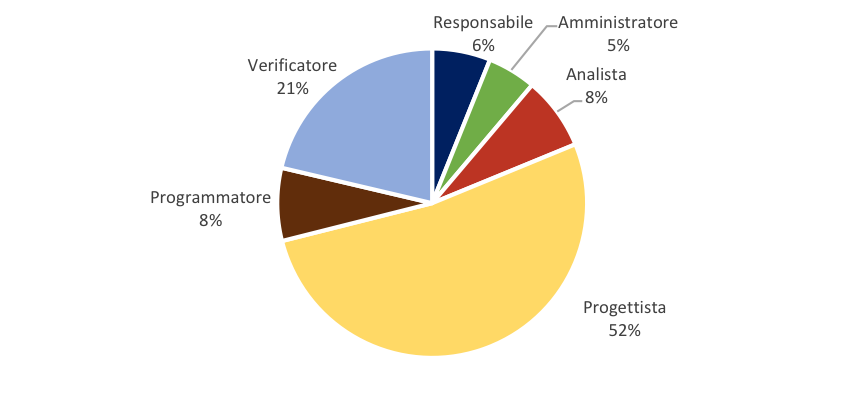
\includegraphics{images/grafoProgettazioneTecnologicaEuro.png}
		\caption{Grafico prospetto orario nel periodo di Analisi dei requisiti in dettaglio}
	\end{center}
\end{figure}
\newpage
\section{Progettazione di Dettaglio e Codifica}
\subsection{Prospetto orario}
Il prospetto orario durante il periodo di Progettazione di Dettaglio e Codifica è illustrato nella seguente tabella:

\begin{table}[!ht]
	\begin{center}
		\begin{tabular}{c}
			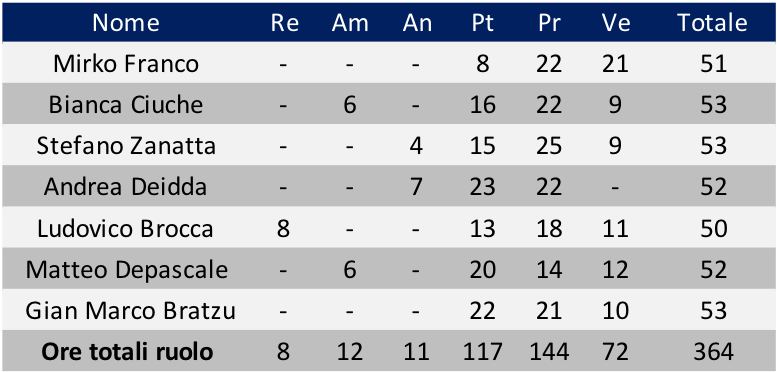
\includegraphics[scale=0.90]{images/tabellaProgettazioneDettaglioCodifica.png}
		\end{tabular}
		\caption{Prospetto orario nel periodo di Progettazione di Dettaglio e Codifica}
	\end{center}
\end{table}

Il seguente grafico mostra una rappresentazione visiva della suddivisione oraria dei ruoli all'interno del gruppo:
\begin{figure}[!ht]
	\begin{center}
		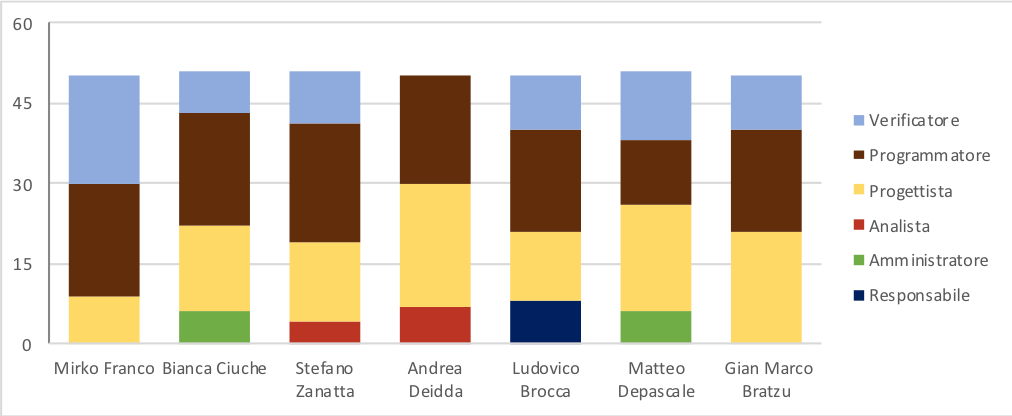
\includegraphics[scale=0.80]{images/grafoProgettazioneDettaglioCodifica.png}
		\caption{Grafico prospetto orario nel periodo di Progettazione di Dettaglio e Codifica}
	\end{center}
\end{figure}

\subsection{Prospetto economico}
Il prospetto economico durante il periodo di Progettazione di Dettaglio e Codifica è illustrato nella seguente tabella:

\begin{table}[!ht]
	\begin{center}
		\begin{tabular}{c}
			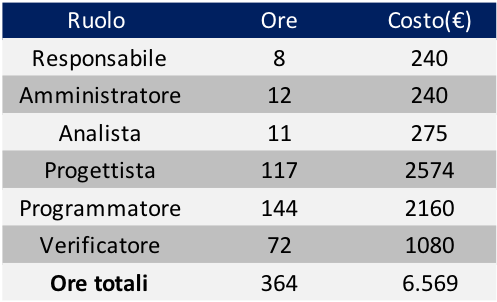
\includegraphics{images/tabellaProgettazioneDettaglioCodificaEuro.png}
		\end{tabular}
		\caption{Prospetto Economico nel periodo di Progettazione di Dettaglio e Codifica}
	\end{center}
\end{table}

\begin{figure}[!ht]
	\begin{center}
		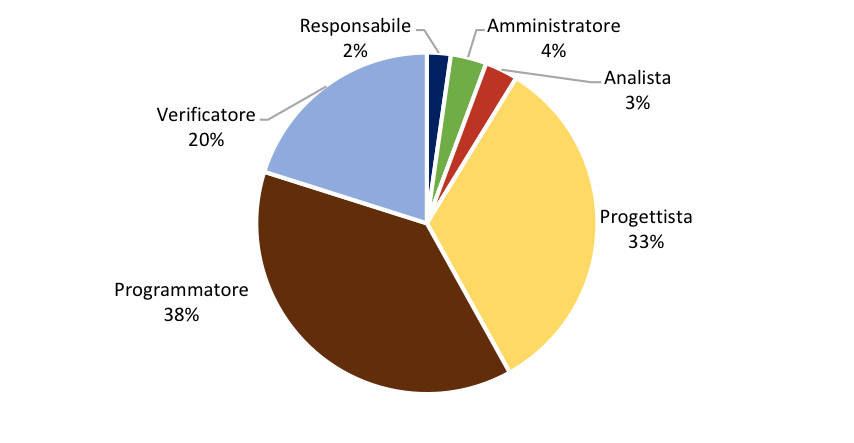
\includegraphics{images/grafoProgettazioneDettaglioCodificaEuro.png}
		\caption{Grafico prospetto economico nel periodo di Progettazione di Dettaglio e Codifica}
	\end{center}
\end{figure}

\newpage
\section{Validazione e Collaudo}
\subsection{Prospetto orario}
Il prospetto orario durante il periodo di Validazione e Collaudo è illustrato nella seguente tabella:

\begin{table}[!ht]
	\begin{center}
		\begin{tabular}{c}
			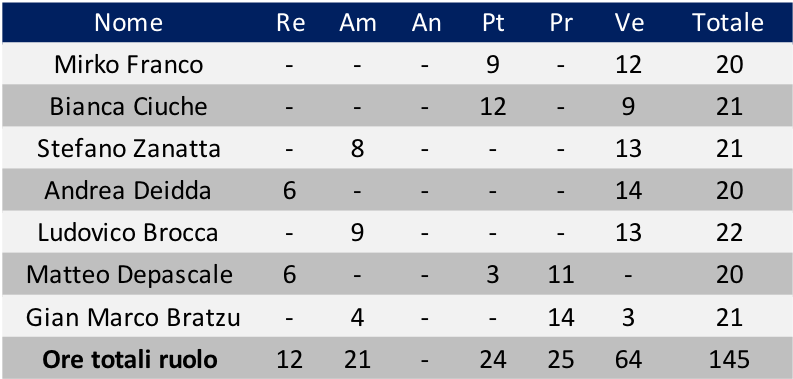
\includegraphics[scale=0.90]{images/tabellaValidazioneCollaudo.png}
		\end{tabular}
		\caption{Prospetto orario nel periodo di Validazione e Collaudo}
	\end{center}
\end{table}

Il seguente grafico mostra una rappresentazione visiva della suddivisione oraria dei ruoli all'interno del gruppo:
\begin{figure}[!ht]
	\begin{center}
		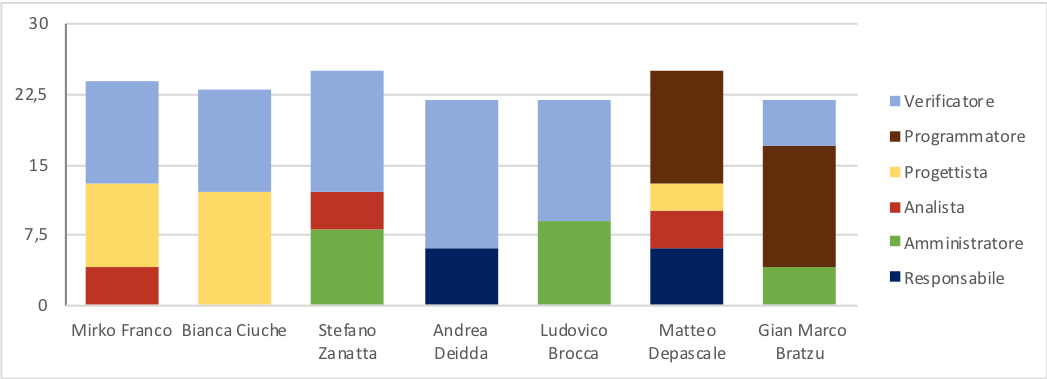
\includegraphics[scale=0.90]{images/grafoValidazioneCollaudo.png}
		\caption{Grafico prospetto orario nel periodo di Validazione e Collaudo}
	\end{center}
\end{figure}

\subsection{Prospetto economico}
Il prospetto economico durante il periodo di Validazione e Collaudo è illustrato nella seguente tabella:

\begin{table}[!ht]
	\begin{center}
		\begin{tabular}{c}
			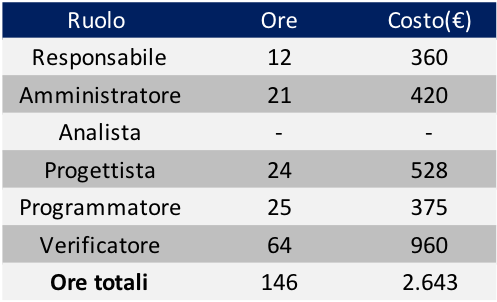
\includegraphics{images/tabellaValidazioneCollaudoEuro.png}
		\end{tabular}
		\caption{Prospetto Economico nel periodo di Validazione e Collaudo}
	\end{center}
\end{table}

La raffigurazione grafica del peso di ogni ruolo sul costo totale è così rappresentata:
\begin{figure}[!ht]
	\begin{center}
		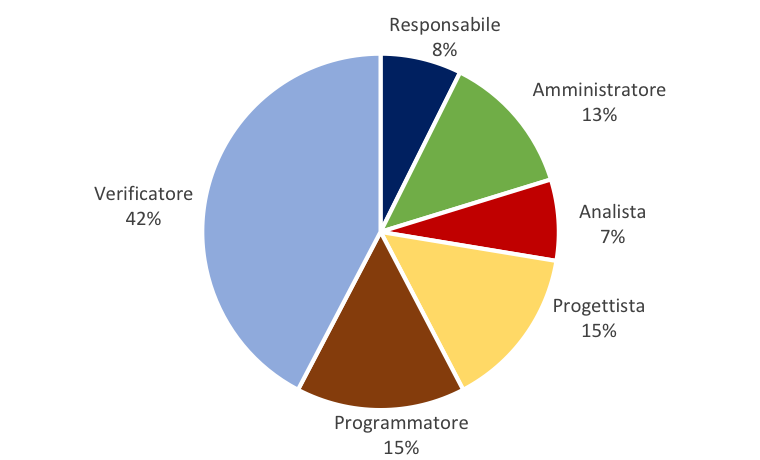
\includegraphics{images/grafoValidazioneCollaudoEuro.png}
		\caption{Grafico prospetto economico nel periodo di Validazione e Collaudo}
	\end{center}
\end{figure}
\newpage
\section{Totale ore rendicontate}
\subsection{Totale del  prospetto orario rendicontato}
Il totale del prospetto orario rendicontato è illustrato nella seguente tabella:

\begin{table}[!ht]
	\begin{center}
		\begin{tabular}{c}
			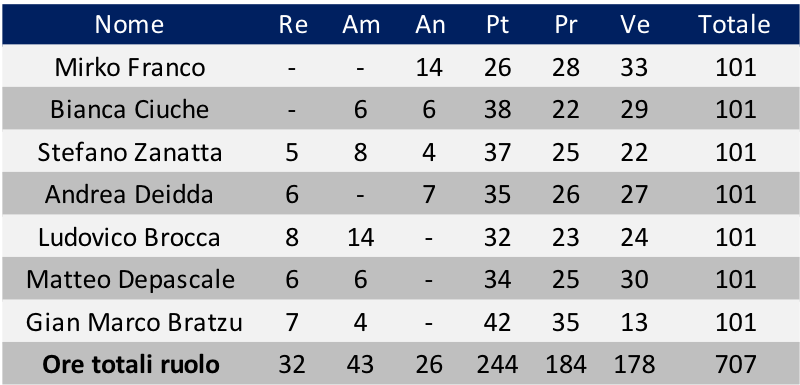
\includegraphics{images/tabellaOreRendicontate.png}
		\end{tabular}
		\caption{Prospetto orario totale delle ore rendicontate}
	\end{center}
\end{table}

Il seguente grafico mostra una rappresentazione visiva della suddivisione oraria dei ruoli all'interno del gruppo:
\begin{figure}[!ht]
	\begin{center}
		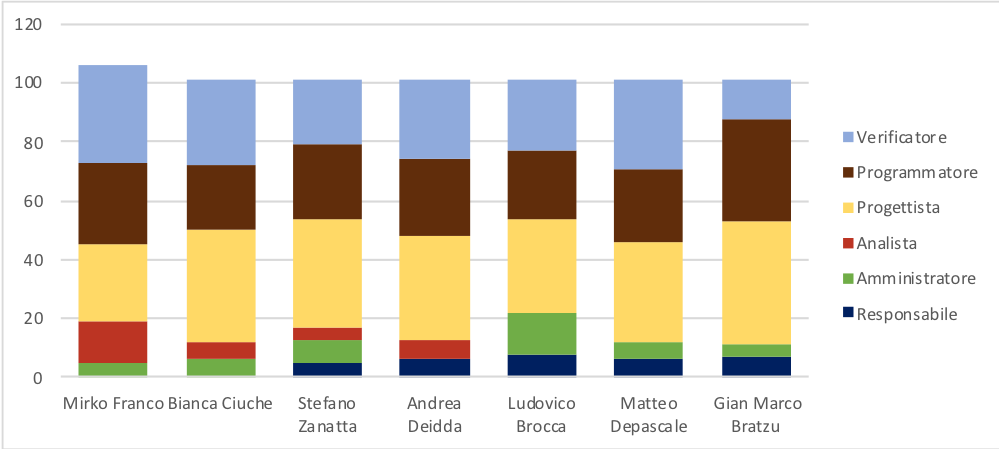
\includegraphics[scale=0.80]{images/grafoOreRendicontate.png}
		\caption{Grafico prospetto orario totale delle ore rendicontate}
	\end{center}
\end{figure}

\subsection{Totale del prospetto economico rendicontato}
Il totale del prospetto economico rendicontato che  include le ore rendicontate nel preventivo a carico del committente cioè dei periodi di Progettazione della Base Tecnologica, Progettazione di Dettaglio e Codifica e il periodo di Validazione e Collaudo è illustrato nella seguente tabella:

\begin{table}[!ht]
	\begin{center}
		\begin{tabular}{c}
			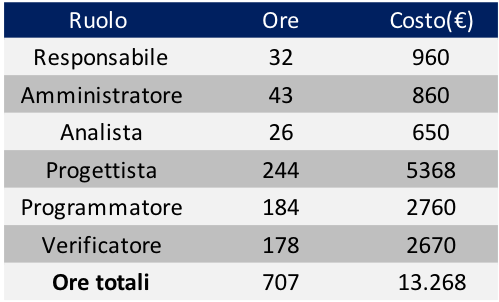
\includegraphics{images/tabellaOreRendicontateEuro.png}
		\end{tabular}
		\caption{Prospetto economico totale delle ore rendicontate}
	\end{center}
\end{table}

La raffigurazione grafica del peso di ogni ruolo sul costo totale è così rappresentata:

\begin{figure}[!ht]
	\begin{center}
		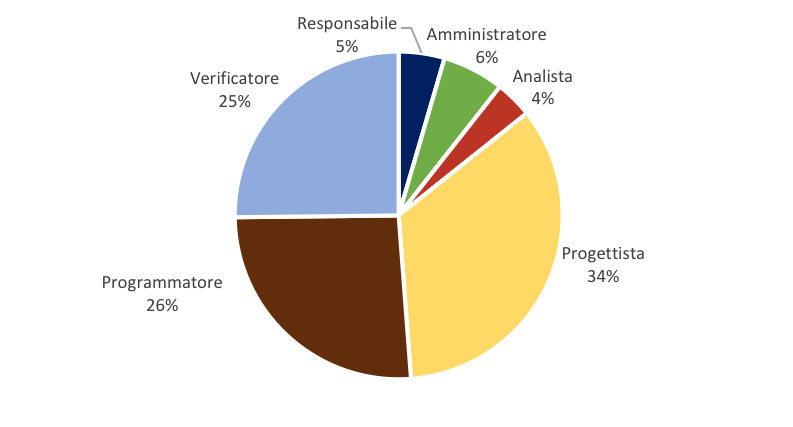
\includegraphics[scale=0.90]{images/grafoOreRendicontateEuro.png}
		\caption{Grafico prospetto economico totale delle ore rendicontate}
	\end{center}
\end{figure}

\section{Totale ore con investimento}
\subsection{Totale del prospetto orario con investimento}
Il totale del prospetto orario con investimento che include sia le ore rendicontate nel preventivo a carico del committente sia le ore di investimento iniziali,è illustrato nella seguente tabella:

\begin{table}[!ht]
	\begin{center}
		\begin{tabular}{c}
			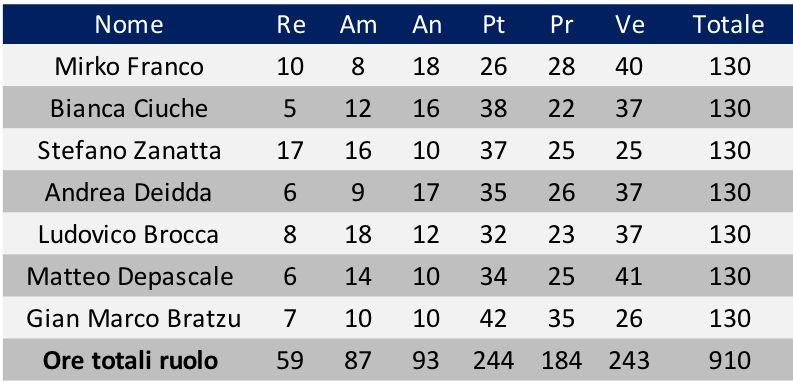
\includegraphics[scale=0.80]{images/tabellaOreInvestimento.png}
		\end{tabular}
		\caption{Prospetto orario totale delle ore di investimento e rendicontate}
	\end{center}
\end{table}

Il seguente grafico mostra una rappresentazione visiva della suddivisione oraria dei ruoli all'interno del gruppo:
\begin{figure}[!ht]
	\begin{center}
		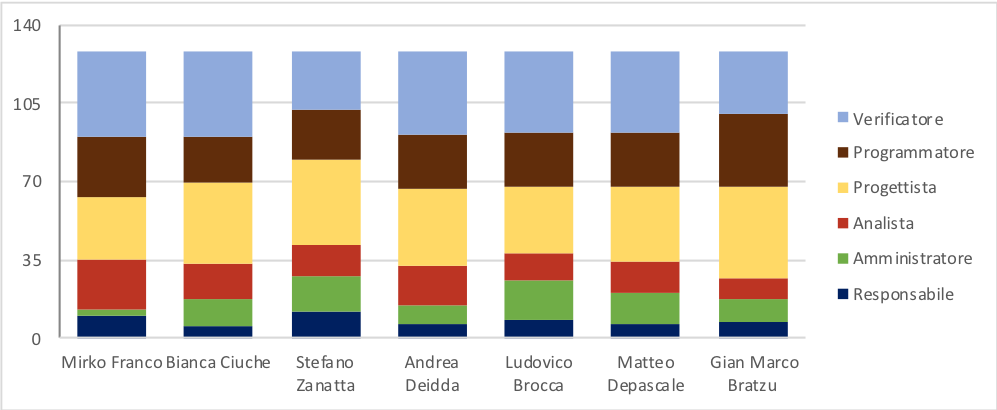
\includegraphics[scale=0.80]{images/grafoOreInvestimento.png}
		\caption{Grafico prospetto orario totale delle ore di investimento e rendicontate}
	\end{center}
\end{figure}

\subsection{Totale del prospetto economico con investimento}
Il totale del prospetto economico con investimento che include sia le ore rendicontate nel preventivo a carico del committente sia  le ore  di investimento iniziali per l'intera durata del progetto è illustrato nella seguente tabella:
\begin{table}[!ht]
	\begin{center}
		\begin{tabular}{c}
			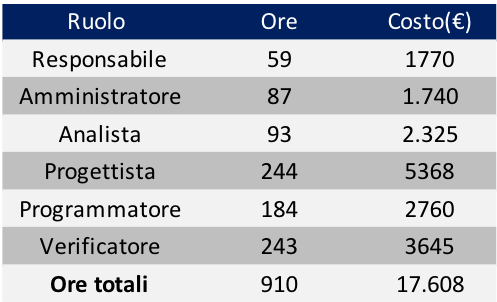
\includegraphics{images/tabellaOreInvestimentoEuro.png}
		\end{tabular}
		\caption{Prospetto economico totale delle ore di investimento e rendicontate}
	\end{center}
\end{table}

La raffigurazione grafica del peso di ogni ruolo sul costo totale è così rappresentata:
\begin{figure}[!ht]
	\begin{center}
		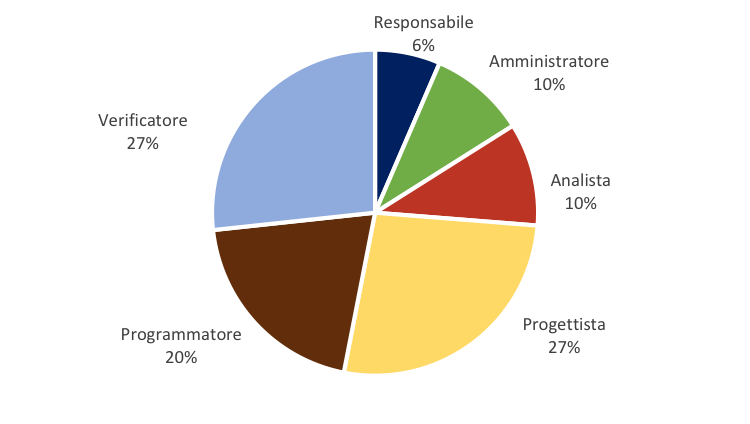
\includegraphics{images/grafoOreInvestimentoEuro.png}
		\caption{Grafico prospetto economico totale delle ore di investimento e rendicontate}
	\end{center}
\end{figure}




	\chapter{Analisi dei rischi}
Per aumentare la probabilità di una buona riuscita del progetto viene effettuata un'approfondita analisi dei rischi. Per poter gestire i rischi viene applicata la seguente procedura:
\begin{itemize}
	\item \textbf{Identificazione:} identificare i potenziali rischi che possono minare l'avanzamento del progetto e capirne la cause. I rischi possono afferire alle seguenti categorie:
	\begin{itemize}
		\item \textbf{Progetto}: relativi alle risorse, alla pianificazione e agli strumenti;
		\item \textbf{Prodotto}: relativi alla conformità del prodotto a quanto atteso dal committente;
		\item \textbf{Mercato}: relativi a costi.
	\end{itemize}
	\item \textbf{Analisi}: ne viene valutata la probabilità di occorrenza, la pericolosità e le possibili conseguenze;
	\item \textbf{Pianificazione}: vengono attuate strategie che permettono di evitare i rischi o mitigarne gli effetti qualora si presentassero;
	\item \textbf{Controllo}: viene posta attenzione continua tramite la rilevazione di specifici indicatori raffinando le strategie di pianificazione qualora ve ne fosse il bisogno.
\end{itemize}
\section{Elenco dei rischi}
Ogni rischio viene classificato secondo la seguente convenzione:\\\\
\centering \textbf{R[Tipo][Identificativo]}\\
\begin{itemize}
	\item La lettera "R" è l'abbreviazione di Rischio
	\item Il secondo valore indica il tipo di rischio. Può essere:
	\begin{itemize}
		\item \textbf{P}: indica i rischi legati al progetto, quindi a risorse, pianificazione e strumenti;
		\item \textbf{PR}: indica i rischi legati ai requisiti;
		\item \textbf{M}: indica i rischi legati al mercato.
	\end{itemize}
	\item L'identificato è semplicemente un numero progressivo.
\end{itemize}
<<<<<<< refs/remotes/origin/feature/PianoDiProgetto
\begin{table}[tbph]
	\caption{Tabella dei rischi}
	\begin{tabularx}{\textwidth}{|X|X|X|X|}
		\hline
		\textbf{Nome} \newline \textbf{Codice} & \textbf{Descrizione} & 	\textbf{Rilevamento} & \textbf{Grado di rischio}\\
		\hline
		
		Scarsa esprienza \newline RP001 & Nessun membro del gruppo ha esperienza in un progetto di tali dimensioni e complessità. &
		Ogni membro comunicherà al Responsabili eventuali difficoltà incontrate. & Occorrenza: Media \newline Pericolosità: Alta \\
		\hline
		\multicolumn{4}{|>{\hsize=\dimexpr4\hsize+4\tabcolsep+\arrayrulewidth\relax}X|}{\textbf{Mitigazione}: Il Responsabile pianificherà le attività cercando di valorizzare capacità e competenze delle singole persone}\\
		\hline

			Scarsa esprienza \newline RP001 & Nessun membro del gruppo ha esperienza in un progetto di tali dimensioni e complessità. &
		Ogni membro comunicherà al Responsabili eventuali difficoltà incontrate. & Occorrenza: Media \newline Pericolosità: Alta \\
		\hline
		\multicolumn{4}{|>{\hsize=\dimexpr4\hsize+4\tabcolsep+\arrayrulewidth\relax}X|}{\textbf{Mitigazione}: Il Responsabile pianificherà le attività cercando di valorizzare capacità e competenze delle singole persone}\\
		\hline
		
			Scarsa esprienza \newline RP001 & Nessun membro del gruppo ha esperienza in un progetto di tali dimensioni e complessità. &
		Ogni membro comunicherà al Responsabili eventuali difficoltà incontrate. & Occorrenza: Media \newline Pericolosità: Alta \\
		\hline
		\multicolumn{4}{|>{\hsize=\dimexpr4\hsize+4\tabcolsep+\arrayrulewidth\relax}X|}{\textbf{Mitigazione}: Il Responsabile pianificherà le attività cercando di valorizzare capacità e competenze delle singole persone}\\
		\hline
		
			Scarsa esprienza \newline RP001 & Nessun membro del gruppo ha esperienza in un progetto di tali dimensioni e complessità. &
		Ogni membro comunicherà al Responsabili eventuali difficoltà incontrate. & Occorrenza: Media \newline Pericolosità: Alta \\
		\hline
		\multicolumn{4}{|>{\hsize=\dimexpr4\hsize+4\tabcolsep+\arrayrulewidth\relax}X|}{\textbf{Mitigazione}: Il Responsabile pianificherà le attività cercando di valorizzare capacità e competenze delle singole persone}\\
		\hline
		
			Scarsa esprienza \newline RP001 & Nessun membro del gruppo ha esperienza in un progetto di tali dimensioni e complessità. &
		Ogni membro comunicherà al Responsabili eventuali difficoltà incontrate. & Occorrenza: Media \newline Pericolosità: Alta \\
		\hline
		\multicolumn{4}{|>{\hsize=\dimexpr4\hsize+4\tabcolsep+\arrayrulewidth\relax}X|}{\textbf{Mitigazione}: Il Responsabile pianificherà le attività cercando di valorizzare capacità e competenze delle singole persone}\\
		\hline
		
			Scarsa esprienza \newline RP001 & Nessun membro del gruppo ha esperienza in un progetto di tali dimensioni e complessità. &
		Ogni membro comunicherà al Responsabili eventuali difficoltà incontrate. & Occorrenza: Media \newline Pericolosità: Alta \\
		\hline
		\multicolumn{4}{|>{\hsize=\dimexpr4\hsize+4\tabcolsep+\arrayrulewidth\relax}X|}{\textbf{Mitigazione}: Il Responsabile pianificherà le attività cercando di valorizzare capacità e competenze delle singole persone}\\
		\hline
		
			Scarsa esprienza \newline RP001 & Nessun membro del gruppo ha esperienza in un progetto di tali dimensioni e complessità. &
		Ogni membro comunicherà al Responsabili eventuali difficoltà incontrate. & Occorrenza: Media \newline Pericolosità: Alta \\
		\hline
		\multicolumn{4}{|>{\hsize=\dimexpr4\hsize+4\tabcolsep+\arrayrulewidth\relax}X|}{\textbf{Mitigazione}: Il Responsabile pianificherà le attività cercando di valorizzare capacità e competenze delle singole persone}\\
		\hline
		
			Scarsa esprienza \newline RP001 & Nessun membro del gruppo ha esperienza in un progetto di tali dimensioni e complessità. &
		Ogni membro comunicherà al Responsabili eventuali difficoltà incontrate. & Occorrenza: Media \newline Pericolosità: Alta \\
		\hline
		\multicolumn{4}{|>{\hsize=\dimexpr4\hsize+4\tabcolsep+\arrayrulewidth\relax}X|}{\textbf{Mitigazione}: Il Responsabile pianificherà le attività cercando di valorizzare capacità e competenze delle singole persone}\\
		\hline
		
		
	\end{tabularx}
\end{table}
=======


\begin{tabularx}{\textwidth}{|X|X|X|X|}
	\caption{Example of an table}\\
	\toprule
	\textbf{Nome} \newline \textbf{Codice} & \textbf{Descrizione} & 	\textbf{Rilevamento} & \textbf{Grado di rischio}\\
	\midrule
	\endhead
	
	Scarsa esprienza \newline RP001 & Nessun membro del gruppo ha esperienza in un progetto di tali dimensioni e complessità. &
	Ogni membro comunicherà al Responsabili eventuali difficoltà incontrate. & Occorrenza: Media \newline Pericolosità: Alta \\
	\hline
	\multicolumn{4}{|>{\hsize=\dimexpr4\hsize+4\tabcolsep+\arrayrulewidth\relax}X|}{\textbf{Mitigazione}: Il Responsabile pianificherà le attività cercando di valorizzare capacità e competenze delle singole persone}\\
	\hline
   
   
   
   Scarsa esprienza \newline RP001 & Nessun membro del gruppo ha esperienza in un progetto di tali dimensioni e complessità. &
   Ogni membro comunicherà al Responsabili eventuali difficoltà incontrate. & Occorrenza: Media \newline Pericolosità: Alta \\
   
   \multicolumn{4}{|>{\hsize=\dimexpr4\hsize+4\tabcolsep+\arrayrulewidth\relax}X|}{\textbf{Mitigazione}: Il Responsabile pianificherà le attività cercando di valorizzare capacità e competenze delle singole persone}\\
	\hline
	Scarsa esprienza \newline RP001 & Nessun membro del gruppo ha esperienza in un progetto di tali dimensioni e complessità. &
	Ogni membro comunicherà al Responsabili eventuali difficoltà incontrate. & Occorrenza: Media \newline Pericolosità: Alta \\
	\hline
	\multicolumn{4}{|>{\hsize=\dimexpr4\hsize+4\tabcolsep+\arrayrulewidth\relax}X|}{\textbf{Mitigazione}: Il Responsabile pianificherà le attività cercando di valorizzare capacità e competenze delle singole persone}\\
	
	Scarsa esprienza \newline RP001 & Nessun membro del gruppo ha esperienza in un progetto di tali dimensioni e complessità. &
	Ogni membro comunicherà al Responsabili eventuali difficoltà incontrate. & Occorrenza: Media \newline Pericolosità: Alta \\
	\hline
	\multicolumn{4}{|>{\hsize=\dimexpr4\hsize+4\tabcolsep+\arrayrulewidth\relax}X|}{\textbf{Mitigazione}: Il Responsabile pianificherà le attività cercando di valorizzare capacità e competenze delle singole persone}\\
	
	 
 

   
    \bottomrule
    \end{tabularx}
>>>>>>> fix tabella

	\begin{flushleft}
    \chapter{Consuntivo di periodo e preventivo a finire}
    Il \textit{Consuntivo di periodo} contiene il prospetto economico che riporta le spese effettivamente sostenute. Vengono riportate le ore impiegate per svolgere i compiti preventivati, sia per
    ruolo che per persona. Il bilancio è ottenuto facendo la differenza di ore tra il preventivo e il consuntivo.\\
    Il bilancio può essere:
    \begin{itemize}
        \item \textbf{Positivo:} se il preventivo ha superato il consuntivo;
        \item \textbf{Negativo:} se il consuntivo ha superato il preventivo;
        \item \textbf{In pari:} se consuntivo e preventivo coincidono.
    \end{itemize}

   \newpage
    \section{Bilancio Analisi}
    La tabella riporta la differenza delle ore tra preventivo e consuntivo, divise per ruolo. Il segno negativo indica che le ore effettive superano le ore preventivate.  
      
	\begin{table}[!h]
		\begin{center}
			\rowcolors{1}{}{lightgray}
			\begin{tabular}{ccc}
				\rowcolor{coolblack}
				\hline
				\textcolor{white}{Ruolo} & \textcolor{white}{Ore} & \textcolor{white}{Costo in \euro}\\
				\hline
				Responsabile   & 22 (-2)  &  660,00 (-60,00) 	\\ 
				Amministratore & 39 (+2)  &  780,00 (+40,00) 	\\ 
				Analista       & 58 (+1)  &  1450,00 (+25,00)   	\\ 
				Progettista    & -  	 &  - 					\\ 
				Verificatore   & 49(-2)  &  735,00 (-30,00) 	\\ 
				Programmatore  & -       &  -    		 		\\ \hline
				\textbf{Totale}& \textbf{168} & \textbf{3625,00}	\\ \hline 
				\textbf{Totale preventivato}& \textbf{167} & \textbf{3600,00}\\ \hline 
				\textbf{Differenza}& \textbf{-1} & \textbf{-25,00 }	\\ \hline  
			\end{tabular}
			\caption{Differenza delle ore tra preventivo e consultivo divise per ruolo} 
		\end{center}
	\end{table}
\newpage
    In questa tabella  sono riportate le differenze tra le ore di lavoro previste per ogni membro del gruppo con quelle realmente impiegate.
       \begin{table}[!h]
 	\begin{center}
 		\rowcolors{1}{}{lightgray}
 		\begin{tabularx}{\textwidth}{|c|cccccc|c|}
 			
 			\hline
 			\multirow{2}{*}{Nominativo} & \multicolumn{6}{c|}{Ore per ruolo} & \multirow{2}{*}{Ore totali} \\ \cline{2-7}
 			& Re & Am & An & Pt & Ve & Pr &      \\ \hline
 			\endhead
 			Mirko Franco       &   &    &  &    &  &  & 0    \\ \hline
 			Bianca Ciuche      & -2 &  & +1 &    &  &   & -1       \\ \hline
 			Stefano Zanatta    &   &  &  &  &   &   &    0   \\ \hline
 			Andrea Deidda      &   & +2 &   &   &  &   &  +2  		\\ \hline
 			Ludovico Brocca    &   &  &  &  & -1 &   & -1       \\ \hline
 			Matteo Depascale   &   &  &   &   &  -1 &  & -1  		\\ \hline
 			Gian Marco Bratzu  &   &  &   &   &  &   & 0        \\ \hline
 			
 		\end{tabularx}
 		\caption{Differenza tra le ore di lavoro previste per ogni membro del gruppo con le ore realmente impiegate }
 		\end{center}
	 \end{table}
    \subsection{Conclusioni}
    La stesura del \textit{Piano di Progetto} ha richiesto più lavoro del previsto da parte dei \textit{Responsabili} e dei \textit{Verificatori}. Il carico di lavoro degli \textit{Amministratori} e degli \textit{Analisti} è stato inferiore di quanto preventivato.\\ Il bilancio totale è negativo, con un deficit di 25\euro. Questo costo non è a carico del committente, in quanto è stato generato dalle attività di Analisi.
    
    \newpage
    
\section{Bilancio Revisione Analisi}\label{BilRevAn}
La tabella riporta la differenza delle ore tra preventivo e consuntivo, divise per ruolo. Il segno negativo indica che le ore effettive superano le ore preventivate.  
  
\begin{table}[!h]
	\begin{center}
		\rowcolors{1}{}{lightgray}
		\begin{tabular}{ccc}
			\rowcolor{coolblack}
			\hline
			\textcolor{white}{Ruolo} & \textcolor{white}{Ore} & \textcolor{white}{Costo in \euro}\\
			\hline
			Responsabile   & 5 (+2)  &  150,00 (+60,00) 	\\ 
			Amministratore & 5 (-3)  &  100,00 (-60,00) 	\\ 
			Analista       & 9 (-5)  &  225,00 (-125,00)   	\\ 
			Progettista    & -  	 &  - 					\\ 
			Verificatore   & 16(+5)  &  240,00 (+75,00) 	\\ 
			Programmatore  & -       &  -    		 		\\ \hline
			\textbf{Totale}& \textbf{37} & \textbf{765,00}	\\ \hline 
			\textbf{Totale preventivato}& \textbf{35} & \textbf{715,00}\\ \hline 
			\textbf{Differenza}& \textbf{-2} & \textbf{-50,00 }	\\ \hline  
		\end{tabular}
		\caption{Differenza delle ore tra preventivo e consultivo divise per ruolo} 
	\end{center}
\end{table}
  \clearpage
In questa tabella  sono riportate le differenze tra le ore di lavoro previste per ogni membro del gruppo con quelle realmente impiegate.\\

    \begin{table}[!h]
	\begin{center}
		\rowcolors{1}{}{lightgray}
		\begin{tabularx}{\textwidth}{|c|cccccc|c|}
			
			\hline
			\multirow{2}{*}{Nominativo} & \multicolumn{6}{c|}{Ore per ruolo} & \multirow{2}{*}{Ore totali} \\ \cline{2-7}
			& Re & Am & An & Pt & Ve & Pr &      \\ \hline
			\endhead
			Mirko Franco       &  & -2  & &  & +1 &   & -1   \\ \hline
			Bianca Ciuche      & +2 &    & -2 &    &  &   & 0   \\ \hline
			Stefano Zanatta    &   & -1 & -2 &  & +1 &  & -2    \\ \hline
			Andrea Deidda      &   &  &   &   & +1  &   & +1	\\ \hline
			Ludovico Brocca    &   &  & -1 &   & +1 &   & 0     \\ \hline
			Matteo Depascale   &   &  &   &   &   &   & 0  		\\ \hline
			Gian Marco Bratzu  &   &  &   &   &  &   & 0        \\ \hline
			
		\end{tabularx}
		\caption{Differenza tra le ore di lavoro previste per ogni membro del gruppo con le ore realmente impiegate }
	\end{center}
\end{table}

  \subsection{Conclusioni}
  Le correzioni del \textit{Piano di Qualifica} e del documento \textit{Norme} ha richiesto più lavoro del previsto agli {Analisti}. Il carico di lavoro degli \textit{Verificatori} è stato inferiore di quanto preventivato.\\ Il bilancio totale è negativo, con un deficit di 50\euro.
  Un'attenta analisi sulle tecnologie ha portato alla decisione di redistribuire le ore preventivate per la progettazione della base tecnologica, in quanto il carico di lavoro risultava squilibrato a favore dei Progettisti e stabiliva poche ore di programmazione.

\newpage	
	\section{Bilancio Progettazione della Base Tecnologica} 
	\label{BilProgBT}
  La tabella riporta la differenza delle ore tra preventivo e consuntivo, divise per ruolo. Il segno negativo indica che le ore effettive superano le ore preventivate.
  
	\begin{table}[!h]
	\begin{center}
		\rowcolors{1}{}{lightgray}
		\begin{tabular}{ccc}
			\rowcolor{coolblack}
			\hline
			\textcolor{white}{Ruolo} & \textcolor{white}{Ore} & \textcolor{white}{Costo in \euro}\\
			\hline
			Responsabile   & 7   		&  210,00  			 	\\ 
			Amministratore & 5   		&  100,00 			 	\\ 
			Analista       & 15 (+4)	  	&  375,00 (+100)   	\\ 
			Progettista    & 101 (+5)	&  2222,00 (+110,00) 	\\ 
			Verificatore   & 34 (+5)  	&  510,00 (+75,00) 		\\ 
			Programmatore  & 15 (-14)   &  225,00 (-210,00) 	\\ \hline
			\textbf{Totale}& \textbf{177} & \textbf{3567,00}	\\ \hline 
			\textbf{Totale preventivato}& \textbf{177} & \textbf{3642,00}\\ \hline 
			\textbf{Differenza}& \textbf{0} & \textbf{+75,00 }	\\ \hline  
		\end{tabular}
		
		\caption{Differenza delle ore tra preventivo e consultivo divise per ruolo} 
	\end{center}
\end{table}
  \clearpage
  
  In questa tabella  sono riportate le differenze tra le ore di lavoro previste per ogni membro del gruppo con quelle realmente impiegate.\\
  
    \begin{table}[!h]
  	\begin{center}
  		\rowcolors{1}{}{lightgray}
    \begin{tabularx}{\textwidth}{|c|cccccc|c|}
  			
  	\hline
  	\multirow{2}{*}{Nominativo} & \multicolumn{6}{c|}{Ore per ruolo} & \multirow{2}{*}{Ore totali} \\ \cline{2-7}
  					  & Re & Am & An & Pt & Ve & Pr &      \\ \hline
  	\endhead
  	Mirko Franco       &   &    &    &    &  &   & 0        \\ \hline
  	Bianca Ciuche      &   &    &    &    &  &   & 0        \\ \hline
  	Stefano Zanatta    &   &    &  & +5 &   & -5  & 0        \\ \hline
  	Andrea Deidda      &   &  &   &   &   &   & 0  		\\ \hline
  	Ludovico Brocca    &   &  &   &   &  &   & 0        \\ \hline
  	Matteo Depascale   &   &  &   &   & -5  & +5  & 0  		\\ \hline
  	Gian Marco Bratzu  &   &  &   &   &  &   & 0        \\ \hline
    
   	\end{tabularx}
  	\caption{Differenza tra le ore di lavoro previste per ogni membro del gruppo con le ore realmente impiegate }
\end{center}
\end{table}
  
  \subsection{Conclusioni}
  Durante il periodo di Progettazione della base tecnologica, il numero di ore preventivate si è dimostrato corretto. Tuttavia è stato necessario ridistribuire le ore a ruoli diversi, poiché per il periodo non è stato necessario utilizzare tutte le ore preventivate per la progettazione della base tecnologica, ma si sono rese necessarie più ore per la programmazione di essa. 
  Il risultato complessivo del periodo è di 0 ore lavorative in meno rispetto al previsto e di un risparmio di 75,00 \euro.
  
  \newpage

  \section{Preventivo a finire}
  La seguente tabella presenta l'attuale preventivo a finire. Nel caso in cui il valore del consuntivo di un determinato periodo non è ancora presente, per il conteggio totale verrà utilizzato il valore del preventivo.
  

  
	\begin{table}[!h]
  
	\begin{center}
  
		\rowcolors{1}{}{lightgray}
  
		\begin{tabular}{ccc}
  
			\rowcolor{coolblack}
  
			\hline
  
			\textcolor{white}{Periodo} & \textcolor{white}{Preventivo in \euro} & \textcolor{white}{Consuntivo in \euro}\\
  
			\hline
  
			Revisione analisi   & 715,00	&  765,00  			 	\\ 
  
			Progettazione della base tecnologica &  3642,00 &  3567,00 \\ 
  
			Progettazione di dettaglio e codifica    & 6404,00  &  -	\\ 
  
			Validazione e collaudo    & 3018,00 & - 	\\ \hline
  
			\textbf{Totale rendicontato}& \textbf{13.779,00} & \textbf{13.754,00}	\\ \hline   
  
		\end{tabular}
  
		\caption{Preventivo a finire} 
  
	\end{center}
  
\end{table}

   \end{flushleft}
			
	\label{LastPage}

\end{document}